\chapter{L'impiego di \emph{mobile GIS} open source in Archeologia}

L'obiettivo di questo appendice è riassumere alcune delle esperienze accumulate negli ultimi anni a proposito della transizione dei sistemi GIS dal laboratorio all'area di scavo su dispositivi portatili, che ha portato ad un evidente snellimento dei tempi di raccolta dei dati.  In questa breve introduzione alla sincronizzazione dei dati tra cantiere e laboratorio si tralasceranno alcuni aspetti tecnici del software, per porre l'accento sugli aspetti più utili ed interessanti nel contesto archeologico.\\

È ampiamente dimostrato quanto l'archeologia stratigrafica sia legata ai metodi informatici per la documentazione, organizzazione, analisi e comunicazione dello scavo archeologico; è tuttavia interessante notare come alcuni passaggi tra queste fasi vadano notevolmente accorciandosi, grazie al contributo dell'ICT ed in particolar modo delle tecnologie open source, o comunque libere\footnote{Con la presente affermazione si intende aderenti ad una delle licenze riconosciute come ``libere'' dalla Free Software Foundation.}.

Un numero sempre maggiore di archeologi decide di adottare software libero per organizzare il \emph{workflow archeologico}, e non è raro che il contributo sempre crescente di molte realtà, in questo grande ``calderone'' del software libero per l'archeologia, porti allo sviluppo di applicazioni all'avanguardia nel settore rispetto ai competitor \emph{closed source}. Allo stato attuale, lo scenario --- non necessariamente futuristico --- della velocizzazione dei processi di rilievo/analisi a livello archeologico e dell'assenza di rivali commerciali simili sul mercato del software chiuso, vede il coinvolgimento di due attori: gvSIG Mobile e Open Mobile IS.\\

Dall'unione di questi software è nato il progetto Tellus. L'idea di Tellus, che si interseca con le esperienze sul campo di Oxford Archaeology, è proprio quella di trasformare dei palmari economici in strumenti di documentazione/comunicazione in tempo reale, con l'obiettivo di trasmettere \emph{al volo} tutti i dati georiferiti dal cantiere di scavo all'ufficio. Questi risultati possono essere ottenuti soltanto progettando un'infrastruttura hardware e software adatta allo scopo, ed utilizzando programmi che supportino tutti i protocolli di comunicazione necessari al trasferimento e sincronizzazione dei dati. Entrambe queste caratteristiche sono facilmente ottenibili dal processo di sviluppo comunitario diffuso in ambito open source.

\section{gvSIG mobile, Open Mobile IS e Tellus}
%\footnote{Ulteriori informazioni a proposito dell'integrazione dei due programmi nel progetto Tellus possono essere reperite in un paper disponibile online ad opera degli autori di Tellus: \href{https://svn.prodevelop.es/public/labs/gvsigmobileonopenmoko/webresources/media/tellus_article_5th_gvsig_conference.pdf}{https://svn.prodevelop.es/public/labs/gvsigmobileonopenmoko/webresources/media/tellus\_article\_5th\_gvsig\_conference.pdf}.}

	gvSIG\footnote{Sito ufficiale: \href{http://www.gvsig.gva.es}{http://www.gvsig.gva.es}} è un programma scritto in Java, multipiattaforma, per la gestione d'informazione geografica (\emph{GIS}) con precisione cartografica, distribuito con licenza GNU GPL. Permette di gestire dati vettoriali e raster e di connettersi a server cartografici con standard OGC\footnote{Proprio questa è una delle principali caratteristiche di gvSIG: l'implementazione di servizi OGC: WMS (\emph{Web Map Service}), WCS (\emph{Web Coverage Service}), WFS (\emph{Web Feature Service}).}. gvSIG è nato nel 2003, quando la Direzione Infrastrutture e Trasporti della Comunità Valenziana ha deciso di realizzare un proprio SIT. Il progetto è finanziato dall'Unione Europea, Fondo europeo di sviluppo regionale (FEDER).
	
	\begin{wrapfigure}{o}{0.35\columnwidth}
		\centering
		\includegraphics[scale=0.3]{img/tellus/3359542225_2f1736a093_o}
		\caption{{\small \label{fig:Layer-gvSIG}Layer vettoriale di edificato urbano all'interno di gvSIG mobile su dispositivo Openmoko.}}
	\end{wrapfigure}

	Recenti sviluppi del programma hanno portato alla creazione di una versione \emph{mobile}\footnote{Sito ufficiale: \href{http://www.gvsig.gva.es/eng/gvsig-mobile}{http://www.gvsig.gva.es/eng/gvsig-mobile}; sito di riferimetno della versione non ufficiale per dispositivi GNU/Linux: \href{http://gvsigmobileonopenmoko.wordpress.com}{http://gvsigmobileonopenmoko.wordpress.com}.}, con funzioni ridotte rispetto a gvSIG, ottimizzata per essere eseguita su dispositivi dotati di sistema operativo GNU/Linux (fino ad ora lo smartphone FIC Openmoko --- in fig.~\ref{fig:Layer-gvSIG}, il tablet Nokia N800/N810 con sistema operativo Maemo --- Debian GNU/Linux, ed ovviamente qualsiasi dispositivo desktop, netbook compresi, con tale sistema operativo).\\

	Open Mobile IS (abbr. OpenMIS) è un progetto open source (licenza GNU GPL v. 2.1) che ha l'obiettivo di fornire un framework con tutti gli strumenti e le API per la creazione di applicazioni mobile. Open Mobile IS, in particolare, mette a disposizione:
	
	\begin{description}
		\item [{database~integrato}] ottimizzato per funzionare con bassi consumi di CPU e RAM;
		\item [{motore~di~sincronizzazione}] che opera tra il database integrato del dispositivo e un database remoto (nel caso archeologico un database geografico PostGIS); il sistema di tracciamento delle modifiche tra i due database è basato su un \emph{numero di sincronizzazione incrementale}; si evita in questo modo di tracciare le modifiche in base alla data, eliminando la necessità che entrambi i dispositivi che ospitano i database abbiano orologi di sistema sincronizzati (caratteristica molto ultile sul cantiere di scavo).
	\end{description}
	
	Dall'integrazione di OpenMIS in gvSIG mobile è nato il progetto Tellus\footnote{Sito ufficiale: \href{http://tellusproject.blogspot.com/}{http://tellusproject.blogspot.com/}}, che unisce le capacità di sincronizzazione e risoluzione dei conflitti dei dati geografici del primo con le caratteristiche GIS del secondo.

\section{Applicabilità pratica}
	La flessibilità del software libero ed in generale il generoso hardware dei dispositivi supportati da gvSIG mobile, precedentemente citati, sono di fondamentale importanza per l'impiego in campo archeologico, considerate:
	
	\begin{itemize}
		\item le dimensioni notevolmente ridotte rispetto ad un laptop o ad un computer desktop;
		\item il costo mediamente contenuto per l'hardware (a cui si aggiunge la gratuità del software);
		\item la notevole autonomia energetica, incrementabile con batterie aggiuntive dal costo relativamente basso;
		\item l'alta connettività (in media tali dispositivi sono dotati di wifi, bluetooth, e supportano connessioni dati GPRS; Openmoko e Nokia N810 hanno un ricevitore GPS integrato);
		\item le porte di comunicazione standard (mini-USB).
	\end{itemize}
	Questi due ultimi punti rivestono un'importanza fondamentale nel lavoro sul campo, soprattutto perché la connettività è il fulcro del nuovo modo di intendere la documentazione dello scavo archeologico.\\

	L'infrastruttura nel suo complesso, raffigurata schematicamente in fig.~\ref{fig:schema_tellus} è costituita da una serie di client (ovvero tutti i dispositivi utilizzati sul campo: palmari, tablet, notebook e netbook, raffigurati sulla sinistra) sui quali è stato installato Tellus, e da un server localizzato nel laboratorio, equipaggiato con sistema operativo GNU/Linux, su cui sono installati MapServer e un database PostGIS (entrambi open source). A questi due fronti di scambio del dato archeologico se ne aggiunge un terzo, quello dei computer degli operatori in ufficio, che collegandosi al database PostGIS sul server possono visualizzare in tempo reale il flusso dei dati dal campo, e quindi lavorare ed elaborare la documentazione ``in diretta''. Tutti gli elementi di questa rete comunicano tra loro tramite una normale connessione ad internet.\\

	Prima dello scavo l'intera cartografia a disposizione, omogeneizzata in un formato compatibile con gvSIG (ad esempio SHAPEfile, ma gli sviluppatori hanno documentato anche l'utilizzo di WKT) e opportunamente divisa in layer, viene caricata sul server. Durante le quotidiane operazioni di documentazione, i fogli quadrettati, i fili a piombo e lo scalimetro vengono sostituiti dai più veloci ed efficienti palmari, netbook e stazione totale; la carta cede il passo ad un layer sul GIS nel palmo della mano dell'operatore. Il dispositivo palmare connesso ad internet scambia in tempo reale informazioni con il server, aggiornando simultaneamente i layer vettoriali e raster.

	Il rilievo viene effettuato:
	
	\begin{enumerate}
		\item con l'utilizzo della stazione totale;
		\item aggiungendo a mano direttamente sul layer del GIS mobile le informazioni.
	\end{enumerate}
	
	Nel primo caso, non sarà necessario arrivare nel laboratorio sul campo per inviare i dati direttamente dalla stazione totale all'ufficio: gli sforzi di Stefano Costa e Luca Bianconi hanno portato alla creazione di Total Open Station\footnote{\href{http://tops.berlios.de/}{http://tops.berlios.de/}}, software (ben integrato con Openmoko) che permette di scaricare i dati direttamente dalla stazione sul palmare, dal quale potrebbero essere eventualmente inviati in ufficio via wifi o GPRS.

	Nel secondo caso, tutte le informazioni rilevate vengono sincronizzate con il server PostGIS via internet (quindi usando una connessione wifi o GPRS laddove possibile) e messe a disposizione dei ricercatori collegati al server PostGIS, teoricamente da qualsiasi punto del mondo.  Se nel server è installato ed opportunamente configurato MapServer, è possibile impostarlo per aggiornare ad intervalli regolari la mappa raster partendo dal database, in maniera tale da poter offrire ai ricecatori connessi un WMS quasi in tempo reale. La configurazione di un eventuale interfaccia web per la visualizzazione del WMS o in generale di cartografia archeologica gode di una tradizione ormai consolidata in ambito open source, grazie all'utilizzo di software come p.mapper o OpenLayers.\\


	Il dispositivo portatile con Tellus non invia solo dati, ma contemporaneamente può riceverne, sia in forma vettoriale che raster, poichè gvSIG integra il supporto al WMS. Il trasferimento dei dati cartografici tra gvSIG mobile, OpenIMS e il server viene effettuato tramite il protocollo SOAP (una specifica XML). Il trasferimento effettivo dei file può avvenire in due maniere:
	
	\begin{itemize}
		\item Via HTTP, l'intero progetto cartografico viene trasferito in un unico archivio.
		\item Via Bittorrent, il palmare funge non solo da client, ma anche da server momentaneo per l'invio dei file cartografici ad altri palmari connessi alla rete, sincronizzando i file sull'intero parco macchine portatile; è raccomandata per la sincronizzazione di grandi quantità di dati, in quanto il torrent ha una migliore gestione della rete e di eventuali disconnessioni improvvise.
	\end{itemize}

\section{Conclusioni}
	Le applicazioni di un sistema di lettura e modifica di dati geografici in tempo reale sono molteplici e difficilmente riassumibili. L'applicabilità nel settore dei beni culturali, e particolarmente in quello archeologico, è limitata soltanto dal dover ottenere connettività sul cantiere di scavo, ma offre il vantaggio di unire i momenti del rilievo e dell'elaborazione dei dati, operazioni effettuate non necessariamente dagli stessi operatori, e non necessariamente nello stesso luogo fisico.

	Si apre al contempo la strada al concetto di \emph{open archaeology}, avvicinando il patrimonio archeologico al cittadino, che se non può fisicamente recarsi sul luogo di scavo, potrebbe osservare l'evoluzione della ricerca archeologica quasi ``in diretta'' via internet; in maniera simile, si potrebbe filtrare l'accesso ai soli addetti ai lavori, o distribuire l'analisi su più punti diversi del territorio, o in più centri di ricerca nel mondo.

	La piena aderenza agli standard \emph{de facto} internazionali dal punto di vista informatico e l'adozione di software open source realizzato in maniera collaborativa, garantiscono la continuità del processo di conoscenza, che in questo frangente diventa il filo conduttore tra Archeologia e Tecnologia.

	\begin{center}
		\begin{figure}
			\centering
			\includegraphics[scale=0.5]{img/tellus/general_scheme}
			\caption{{\small \label{fig:Schema-riassuntivo}Schema riassuntivo del funzionamento di OpenMIS, come struttura di collegamento tra gvSIG mobile e un server PostGIS.}}
		\end{figure}
	\end{center}

	\begin{center}
		\begin{figure}
			\centering
			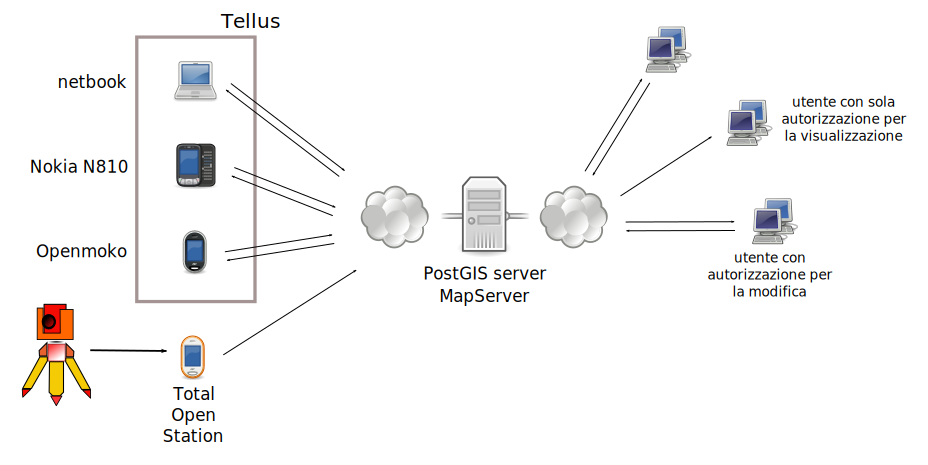
\includegraphics[scale=0.6]{img/tellus/schema_tellus}
			\caption{\label{fig:schema_tellus}{\small Raffigurazione schematica di un'infrastruttura di GIS mobile atta all'impiego in ambito archeologico.}}
		\end{figure}
	\end{center}
